%\documentclass[12pt]{article}
\documentclass[a4paper]{article}
\usepackage{amsmath,amsfonts,amssymb}
\usepackage[utf8]{inputenc}
\usepackage{graphicx}
\usepackage{verbatim}
\usepackage{float}
\usepackage[makeroom]{cancel} %
\usepackage[english]{babel}
\usepackage{textcomp}
\usepackage{gensymb} %
\usepackage{color}
\usepackage{subcaption}
\usepackage{caption}
%\usepackage{hyperref}
%\usepackage{physics}
%\usepackage{dsfont}
%\usepackage{amsfonts}
\usepackage{listings}
\usepackage{multicol}
\usepackage{units}
\usepackage{bm}

% From Eirik's .tex
\usepackage{epstopdf}
\usepackage{cite}
\usepackage{braket}
\usepackage{url}
\bibliographystyle{unsrt}

\usepackage{algorithmicx}
\usepackage{algorithm}% http://ctan.org/pkg/algorithms
\usepackage{algpseudocode}% http://ctan.org/pkg/algorithmicx

\usepackage[margin=1cm]{caption}
\usepackage[outer=1.2in,inner=1.2in]{geometry}

% Finding overfull \hbox
\overfullrule=2cm

\lstset{language=IDL}
 %\lstset{alsolanguage=c++}
\lstset{basicstyle=\ttfamily\small}
 %\lstset{backgroundcolor=\color{white}}
\lstset{frame=single}
\lstset{stringstyle=\ttfamily}
\lstset{keywordstyle=\color{red}\bfseries}
\lstset{commentstyle=\itshape\color{blue}}
\lstset{showspaces=false}
\lstset{showstringspaces=false}
\lstset{showtabs=false}
\lstset{breaklines}
\lstset{aboveskip=20pt,belowskip=20pt}

\lstset{basicstyle=\footnotesize, basewidth=0.5em}
\lstdefinestyle{cl}{frame=none,basicstyle=\ttfamily\small}
\lstdefinestyle{pr}{frame=single,basicstyle=\ttfamily\small}
\lstdefinestyle{prt}{frame=none,basicstyle=\ttfamily\small}
% \lstinputlisting[language=Python]{filename}


\definecolor{codepurple}{rgb}{0.58,0,0.82}
\definecolor{backcolour}{rgb}{0.95,0.95,0.92}
\definecolor{dkgreen}{rgb}{0,0.6,0}
\definecolor{gray}{rgb}{0.5,0.5,0.5}
\definecolor{magenta}{rgb}{0.58,0,0.82}

\lstdefinestyle{pystyle}{
  language=Python,
  aboveskip=3mm,
  belowskip=3mm,
  columns=flexible,
  basicstyle={\small\ttfamily},
  backgroundcolor=\color{backcolour},
  commentstyle=\color{dkgreen},
  keywordstyle=\color{magenta},
  numberstyle=\tiny\color{gray},
  stringstyle=\color{codepurple},
  basicstyle=\footnotesize,
  breakatwhitespace=false,
  breaklines=true,
  captionpos=b,
  keepspaces=true,
  numbers=left,
  numbersep=5pt,
  showspaces=false,
  showstringspaces=false,
  showtabs=false,
  tabsize=2
}

\lstset{language=[90]Fortran,
  basicstyle=\small\ttfamily,
  keywordstyle=\color{red},
  commentstyle=\color{blue},
  stringstyle=\color{dkgreen},
  morecomment=[l]{!\ },
  numbers=left,
  numbersep=5pt
}

%%%%%%%%%%%%%%%%%%%%%%%%%%%%%%%%
% Self made macros here yaaaaaay
\newcommand\answer[1]{\underline{\underline{#1}}}
\newcommand\pd[2]{\frac{\partial #1}{\partial #2}}
\newcommand\red[1]{\textcolor{red}{\textbf{#1}}}
\newcommand\numberthis{\addtocounter{equation}{1}\tag{\theequation}}
% Usage: \numberthis \label{name}
% Referencing: \eqref{name}

% Some matrices
\newcommand\smat[1]{\big(\begin{smallmatrix}#1\end{smallmatrix}\big)}
\newcommand\ppmat[1]{\begin{pmatrix}#1\end{pmatrix}}

%%%%%%%%%%%%%%%%%%%%%%%%%%%%%%%%%
% Eirik's self made macros
\newcommand{\s}{^{*}}
\newcommand{\V}[1]{\mathbf{#1}}
\newcommand{\husk}[1]{\color{red} #1 \color{black}}
\newcommand{\E}[1]{\cdot 10^{#1}}
\newcommand{\e}[1]{\ \text{#1}}
\newcommand{\tom}[1]{\big( #1 \big)}
\newcommand{\Tom}[1]{\Big( #1 \Big)}
\newcommand{\tomH}[1]{\big[ #1 \big] }
\newcommand{\TomH}[1]{\Big[ #1 \Big]}
\newcommand{\tomK}[1]{ \{ #1 \} }
\newcommand{\TomK}[1]{\Big\lbrace #1 \Big\rbrace}
\newcommand{\bigabs}[1]{\left| #1 \right|}

% Practical macros for FYS-STK4155
\newcommand{\XX}{\mathbf{X}}
\newcommand{\II}{\textbf{I}}
\newcommand{\T}{\mathsf{T}}

\newcommand{\Ey}{\mathbb{E}[\bm{\tilde y}]}
\newcommand{\xx}{\mathbf{x}}
\newcommand{\ee}{\bm{\epsilon}}
\newcommand{\yy}{\bm{\tilde y}}
\newcommand{\pr}{\text{Pr}}
\newcommand{\Nepochs}{N_{\text{epochs}}}
\newcommand{\Nbs}{N_{\text{bs}}}
\newcommand{\Nhn}{N_{h,\text{nodes}}}
\newcommand{\Nhl}{N_{h,\text{layers}}}


% Section labeling
%\usepackage{titlesec}% http://ctan.org/pkg/titlesec
%\renewcommand{\thesubsection}{\arabic{subsection}}

% Title/name/date
\title{FYS-STK4155: Project 3}
\author{Simen Nyhus Bastnes}
\date{16. December 2020}

\begin{document}
\maketitle
%%%%%%%%%%%%%%%%%%%%%%%%%%%%%%%%%%%%%%%%%%%%%%%%%
\begin{abstract}
In this project, we want to take a look at audio classification using different machine learning algorithms. The data set we will be looking at is a set of labeled audio files containing either cat or dog sounds. To reduce the complexity of the data set, we transform it into Fourier space, using the binned frequencies as our predictors. Principal component analysis (PCA) is employed to further reduce the predictor set. The classification methods we will be using is a feed-forward neural networks, random forests, and XGBoost. In order to find the optimal hyperparameters we employ grid search with cross-validation.% Cross-validation will be used in order to find the optimal hyperparameters.
%We find that \red{insert results}
%\red{Better at cats, worse at dogs}
% SPECIEST!!!
We find that neural nets and random forest classify the samples with an accuracy of around 90\% for both the normal data set and the reduced data set, with a slight reduction in the PCA reduced results. XGBoost performs the best with almost 95\% accuracy on the full data set, and 93\% on the reduced. Further, we find that the neural net is better at classifying dogs than cats, while random forests and XGBoost classifies cats better. Random forest and XGBoost far outclasses the neural net speed wise, with random forests being almost 3 times faster than XGBoost for the full data set, but slightly slower than XGBoost for the reduced one.

%We find that all three methods classify the samples with an accuracy of over 90\%, with XGBoost performing the best \red{at 95\%}. For all methods there is a slightly lower accuracy rate for classifying dog samples compared to cats, possibly stemming from the larger variance in spectral characteristics between small and large dogs. \red{PCA}
%In this project, we want to study a few methods commonly used in data science for both normal regression problems, as well as classification problems. The methods we will be employing are the stochastic gradient descent (SGD) and feed-forward neural networks (FFNN). For regression, we will be looking at is the Franke function studied in the previous project \cite{Github1}, comparing our results to the ones found there. For classification the MNIST database of handwritten digits will be studied. Cross-validation will be used for the hyperparameter search for both problems in order to make sure the model is the optimal one.

\end{abstract}
%%%%%%%%%%%%%%%%%%%%%%%%%%%%%%%%%%%%%%%%%%%%%%%%%%%%%%%%%%%%%%%%%%%%%%%%%%%%%%%%%%%%%%%%%%
%%%%%%%%%%%%%%%%%%%%%%%%%%%%%%%%%%%%%%%%%%%%%%%%%%%%%%%%%%%%%%%%%%%%%%%%%%%%%%%%%%%%%%%%%%
\section{Introduction}
While image recognition with machine learning seems to have taken the spotlight in recent years when it comes to popularity, using machine learning for audio analysis is a field with a plethora of real world applications, both for supervised and unsupervised learning. Everything from speech recognition to make the lives of deaf individuals easier, to studying seismic data to detect earthquakes, or detect wear in critical machinery at a factory based on the sound or vibrations it makes.
%One of the fields where machine learning is up and coming / with many real world applications is audio analysis. Speech, music, (different waves, earthquakes, sensor data etc.)
%
%Using machine learning algorithms for audio classification is something with many potential real world applications.
%In the last two decades, computation power and availability of said machines has increased drastically, making it possible to employ more and more complex methods of solving both regression and classification problems.
\\\\
In this project, we will be looking at a fairly simple supervised approach for classifying different audio events, namely looking at the Fourier transform of our audio samples. Under the assumption that different types of sound events has different spectral characteristics, we extract a number of features from each sample by binning the frequencies into 40 Hz bins. The methods used for the classification is a standard feed-forward neural network, random forests, and the XGBoost gradient boosting.
\\\\
%We also employ a common dimensionality reduction method, namely the principal component analysis (PCA) in order to te
Since it is unlikely that all the different frequency bins are necessary for our analysis, we also test a common dimensionality reduction method, the principal component analysis (PCA), in order to see how much it affects both the results and run time of our code.
%
%Automatic environmental sound classification is a growing area of research with numerous real world applications. Whilst there is a large body of research in related audio fields such as speech and music, work on the classification of environmental sounds is comparatively scarce.
%Likewise, observing the recent advancements in the field of image classification where convolutional neural networks are used to to classify images with high accuracy and at scale, it begs the question of the applicability of these techniques in other domains, such as sound classification.
%There is a plethora of real world applications for this research, such as:
%• Content-based multimedia indexing and retrieval
%• Assisting deaf individuals in their daily activities
%• Smart home use cases such as 360-degree safety and security capabilities
%• Industrial uses such as predictive maintenance
%
%In this project, we will be looking at two different methods of performing regression and classification, and see how they compare against each other. For regression, we can also compare to the results we found in Project 1 %\cite{Github1}. 
%The methods we will be looking at is the stochastic gradient descent and a feed-forward neural network. These methods contain a few hyperparameters that will need to be adjusted in order to find the best model. In order to remove some dependency on the exact training/test data split, we will employ $k$-fold cross-validation during the hyperparameter search.
\\\\
The data set we will be using is a set of audio files with cat and dog sounds from \cite{Kaggle_catdog}, consisting of 277 samples. As the data set is quite varied in terms of content and quality, this serves as a decent real world test case.
%The data sets we will be looking at is the Franke function from \cite{Franke}, as well as a reduced MNIST data set \cite{MNIST} consisting of approximately 1800 handwritten digits.
First, in Chapter \ref{chap:theory} we will go through the relevant theory, going briefly  through feed-forward neural networks, and then decision trees/random forests, gradient boosting and finally PCA. A more in-depth description of the data sets can be found in Chapter \ref{chap:data_sets}. Then, in Chapter \ref{chap:results} we go through the results of performing the analysis on both the full data set as well as the dimensionality reduced one, while discussing them. Finally, we conclude our findings in Chapter \ref{chap:conclusion}.


%%%%%%%%%%%%%%%%%%%%%%%%%%%%%%%%%%%%%%%%%%%%%%%%%%%%%%%%%%%%%%%%%%%%%%%%%%%%%%%%%%%%%%%%%%
%%%%%%%%%%%%%%%%%%%%%%%%%%%%%%%%%%%%%%%%%%%%%%%%%%%%%%%%%%%%%%%%%%%%%%%%%%%%%%%%%%%%%%%%%%
\section{Theory} \label{chap:theory}
In this chapter we will be going through the fundamentals of the classification methods we will employ, as well as the dimensionality reduction and different metrics we use to gauge how well our models work. For the discussion on decision trees and random forests, we will follow chapter 6 and 7 of \cite{Geron}.
%\red{Logistic regression with softmax check aurelion geron page 195ish}
%For the derivation of the OLS method, Ridge, and Lasso regression, we will follow Chapter 2.3 and 3.4 of Hastie et al. \cite{Hastie}
\subsection{Feed-forward neural network} \label{sec:ffnn}
In this report, we will be using feed-forward neural networks to compare our results with the random forest and gradient boosting methods. A description of how FFNNs function and is trained can be found in \cite{Github2}. Instead of using the neural net we created in project 2, we will be using Scikit-Learns \texttt{MLPClassifier} \cite{MLPClassifier}. In addition to the hyperparameters we tested previously in \cite{Github2}, we will be testing the different solvers SKL has for weight optimization. Besides the stochastic gradient descent, \texttt{MLPClassifier} has a solver in the family of quasi-Newton methods, which is claimed to converge faster and perform better for small datasets.

%\red{go quickly through and mention relevant things + refer to project 2}
%\cite{Github2}
%Mention solvers for the MLPClassifier and that we test them (lbfgs good for small datasets)

\subsection{Decision trees} \label{sec:dec_tree}
Decision trees is a powerful machine learning algorithm that can be used for both regression and classification. One of the strengths of decision trees is the inherent simplicity when it comes to when it comes to understanding how it works. Unlike ANNs or other black box models, decision trees are white boxes, making it easy to interpret why the model makes the prediction. Decision trees are also the fundamental building blocks for both of the ensemble methods (random forest and XGBoost) that we will use later.
\\\\
The base concept of decision trees is that the data set is split into two based on some question/"decision", which can for example be whether or not a person is male or female, or if their height is above or below some 1.7 meters. This process is repeated until all samples are correctly classified or you reach some specified stopping criteria.
\\\\
Figure \ref{fig:iris} shows an example of a decision tree attempting to classify iris flowers based on the sepal and petal length/width. The starting point is the \textit{root node} (depth=0), and the method tries to find the question that separates the data the best. In this case, the question whether or not the petal width is less than or equal to 0.8 cm separates the data best. The left child node (at depth=1) is \textit{pure}, as only samples of a single class is included. Thus, this is a \textit{leaf node}, and there is no reason to split further. The right child node only correctly classifies 50\% of the samples, and needs to be branched again. With a split at petal width $<= 1.75$ cm, the tree separates the data almost fully.
\begin{figure}[H]
	\centering
	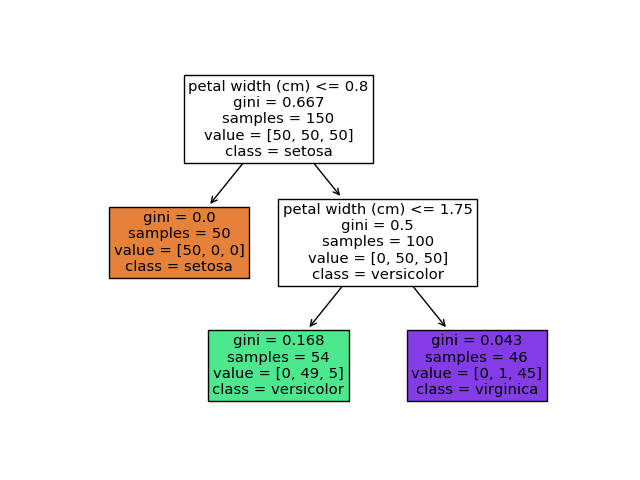
\includegraphics[scale=0.8]{../figures/iris_decision_tree.png}
	\caption{Decision tree example using the Iris data set. Corresponds to figure 6-1 in \cite{Geron}.}
	\label{fig:iris}
\end{figure}	
In order to quantify how pure a node is, we compute the \textit{impurity} of each of the nodes. One of the common ways to do this for classification trees is the so-called Gini score/impurity
\begin{align*}
	G_i &= 1 - \sum_{k=1}^n p_{i,k}^2
\end{align*}
where $p_{i,k}$ is the ratio of class $k$ instances among the training instances in the $i^{\text{th}}$ node. A fully pure node will have a gini score of 0. 
%Alternatively one can use the entropy
%\begin{align*}
%	H_i &= \begin{cases} 
%		-\sum_{k=1}^n p_{i,k}\log(p_{i,k}) & \text{if $p_{i,k} \neq 0$} \\
%		0 & \text{if $p_{i,k} = 0$}
%		\end{cases}
%\end{align*}
\\\\
To train/grow the decision tree, we will look at the CART\footnote{"\textit{Classification and
Regression Tree}"} algorithm as it is the one that Scikit-Learn uses. The algorithm splits the data set into two subsets using a single feature $k$ and a threshold $t_k$, and searches for the pair of ($k$, $t_k$) that yields the purest subsets. The cost function that it tries to minimize is the following
\begin{align*}
	J(k, t_k) &= \frac{m_{\text{left}}}{m}G_{\text{left}} + \frac{m_{\text{right}}}{m}G_{\text{right}}
\end{align*}
where $G_{\text{left/right}}$ is the impurity of the left/right subset, and $m_{\text{left/right}}$ is the amount of instances in the left/right subset, meaning that the impurity is weighted by the size of each subset. It then splits each subset in two following the same logic, continuing until it either cannot find any splits that decrease the impurity, or some stopping criterion is met. One of these criteria is the maximum depth, limiting how deep the tree can go. Some of the hyperparameters that Scikit-Learn has that can be used to tweak how the tree grows is
\begin{itemize}
	\item\texttt{max\_depth}: maximum depth of the tree
	\item\texttt{max\_features}: maximum amount of features to consider when looking for the best split
	\item\texttt{max\_leaf\_nodes}: maximum number of leaf nodes
	\item\texttt{min\_samples\_split}: minimum number of samples required to split
	\item\texttt{min\_samples\_leaf}: minimum number of samples required to be a leaf node
\end{itemize}
As decision trees make very few assumptions about the training data, it can easily end up overfitting, and give very poor results for the test data. Thus, using the different hyperparameters discussed above can help regularize the model and reduce the overfitting. 
Decision trees are also very sensitive to small variations in the training set, making just small variations in the train/test split enough to change your model. This brings us to the next topic, ensemble methods, which attempts to limit this instability aggregating multiple predictions.% of many predictions.
%\red{No feature normalization needed}
%\\\\
%\red{you can fit it extremely well to train data, asking many questions and including all data, but that leads to overfitting, which is why random forests are good}


%\begin{algorithm}[H]
%\caption{Stochastic Gradient descent}
%\begin{algorithmic}[1]
%%\State Given $\XX$, $y$, $\beta^{(0)}$, $\eta$
%\For{$i = 0$, $N_{\text{epochs}}-1$}
%\State Shuffle $\XX_{\text{train}}$ and $y_{\text{train}}$
%\State Split into $N_{\text{mb}}$ minibatches
%\For{$j=0$, $N_{\text{mb}}$}
%\State Compute gradient using minibatch $j$
%\State Update $\beta$
%\EndFor
%%\State (Update learning rate $\eta$ if not using constant learning rate)
%%\State $\beta^{(i+1)} = \beta^{(i)} - \eta \nabla_i$
%\EndFor
%\end{algorithmic}
%\label{alg:sgd}
%\end{algorithm}

\subsection{Ensemble methods} \label{sec:ensemble}
Ensemble learning is a machine learning method where you combine the results of multiple methods to obtain better predictive power than each of the methods alone. While you could combine the results from all kinds of different machine learning algorithms, we will focus on methods based on decision trees, namely random forests as well as look at gradient boosting via the XGBoost library.
\\\\
With ensemble methods even if the classifiers are weak learners (as in a classifier that is only slightly better than random guesses), the ensemble can still be a strong learner, provided there is a large enough and diverse set of classifiers.
%As mentioned earlier, decision trees are good at fitting the training data, but struggles when making predictions on unseen samples. To minimize this problem, we want to look at the aggregated results of While you could combine the results from all kinds of different machine learning algorithms, we will focus on random forests as well as look at gradient boosting via the XGBoost library.
%Decision
%Decision trees good at fitting training data, but struggles with new data/unseen samples (test data). Weak learners, ensemble of them, yes!
\subsubsection{Random forests} \label{sec:random_forest}
The Random Forest is an ensemble method where we train a set of decision trees, and combine the predictions from all the trees to get our final predictions. In order to make our ensemble method as good as possible, we can train each of the decision trees on a different random subset of the training data. Using bootstrap for this is referred to as \textit{bagging} (bootstrap aggregating), while sampling without replacement is referred to as \textit{pasting}.
\\\\
When making the predictions, one can use either \textit{hard} or \textit{soft} voting. Hard voting is simply majority rule, where the class that has the most predictions/votes is the final prediction. Soft voting on the other hand, takes the average of the prediction probabilities for each of the decision trees, and makes the largest one the final prediction. This can give better results than hard voting as it gives more weight to highly confident predictions.
\\\\
The random forest has mostly the same hyperparameters as decision trees, but also how many decision trees to grow, as well as other ensemble parameters. Another benefit with random forests is that instead of searching for the best feature to split at for each node, one can consider a random subset of the features, resulting in greater diversity among the trees and lower variance, producing better results.

\subsubsection{Gradient boosting / XGBoost} \label{sec:xgboost}
Gradient boosting is another ensemble method where you sequentially add more predictors to the ensemble, with each one correcting the predecessor. The way this is done is that we initialize an estimate to our targets. Given a cost function, we compute the negative gradient vector with respect to the previous prediction. Then, we fit our model to the negative gradient, and update the estimate by adding the gradient to the previous estimate. This is done for however long we want, and return our final estimate.
%Omae wa mou shindeiru
\\\\
In this report, we will be using the XGBoost library \cite{Chen_2016} to perform gradient boosting. XGBoost is an optimized distributed gradient boosting library designed to be highly efficient, flexible and portable. It has become an extremely popular library, and has been used to win many machine learning competitions.
%\\\\
%\red{Hyperparameters?}

\subsection{Principal component analysis} \label{sec:pca}
At its core, dimensionality reduction involves transforming data to a space with lower dimensionality than the original. Ideally, this new representation of the data retains as much of the information in the data set as possible, however some loss will always occur. Technically, when defining our data set, as described later in Chapter \ref{chap:data_sets}, we perform a somewhat arbitrary dimensionality reduction when binning the audio frequencies, hoping it works okay. To further reduce the number of dimensions, we employ a much used dimensionality reduction method, namely the principal component analysis (PCA).
\\\\
Principal component analysis works by finding the hyperplane that lies closest to the data, and then projects the data onto it. First, it finds the axis that accounts for the largest amount of variance in the data (the first principal component). Then, the second is the axis orthogonal to the first that maximizes the variance, and so on for the amount of dimensions in the data set (or for as many dimensions you want to compute / reduce the data set to).
\\\\
To compute the principal components, one can for example use singular value decomposition (SVD) to decompose the data matrix into
\begin{align*}
	\XX &= U\Sigma V^\T
\end{align*}
where $V$ contains the principal components. The data set can then be projected down to $D$ dimensions by transforming $\XX$ using the first $D$ components of $V$
\begin{align*}
	\mathbf{T}_D &= \XX V_D
\end{align*}
When determining the amount of dimensions to reduce down to, we can determine how much of the variance to keep, and then set $D$ as the number of principal components needed to retain for example 95\% of the data set variance.
\\\\
One of the issues with this method of performing PCA is that the entire data set $\XX$ needs to fit into memory, which while is not a big problem for our data set, can be difficult with larger data sets. To circumvent this issue, one can for example use an incremental PCA (IPCA) algorithm where the data set is split into mini-batches, or a stochastic approach where an approximation of the principal components is found.

\subsection{Performance metrics} \label{sec:metrics}
To measure the performance of our classifiers, we use a couple of different metrics. First of all, the \textbf{accuracy} gives us the number of correctly guessed
targets $t_i$ divided by the total number of targets.
\begin{align*}
	\text{Accuracy} &= \frac{\sum_{i=1}^n I(t_i = y_i)}{n}
\end{align*}
where $I$ is the indicator function, and $y_i$ is the output from our classifier.
\\\\
For a 2-class classification problem, the correct guesses (for a positive result) can be expressed as the true positive (TN), while the samples incorrectly guessed as positive is the false positive (FP). Likewise with negative results, we have the true negative (TN) and false negative (FN). With this, the accuracy can be written as
\begin{align*}
	\text{Accuracy} &= \frac{\text{TP} + \text{TN}}{n}
\end{align*}
where $n$ is the total amount of samples. To more closely study how our model performs for each class, we plot the \textbf{confusion matrix}
\begin{align*}
	\text{confusion matrix} &= \ppmat{\text{TP} & \text{FP} \\ \text{FN} & \text{TN}}
\end{align*}
for practicality, we can normalize each row, making the values the ratio of true and false positives/negatives.
%The accuracy can also be written in terms of 
Finally, we can plot the true positive rate (TPR)
\begin{align*}
	\text{TPR} &= \frac{\text{TP}}{\text{TP}+\text{FN}}
	\intertext{against the false positive rate (FPR)}
	\text{FPR} &= \frac{\text{FP}}{\text{FP}+\text{TN}}
\end{align*}
at various thresholds to get the so-called \textbf{receiver operating characteristic} (\textbf{ROC}) curve. The area under the ROC curve (\textbf{AUC}) is often used for comparing different methods, but it is worth keeping in mind that it is not a perfect estimator, especially not for small sample sizes \cite{roc_auc}.

% can be used to compare the different classification methods, though 
%The ROC curve is created by plotting the true positive rate (TPR) against the false positive rate (FPR) at various threshold settings
%\red{ROC, cumulative gain}
%https://github.com/CompPhysics/MachineLearning/blob/master/doc/HandWrittenNotes/NotesSeptember24.pdf

%%%%%%%%%%%%%%%%%%%%%%%%%%%%%%%%%%%%%%%%%%%%%%%%%%%%%%%%%%%%%%%%%%%%%%%%%%%%%%%%%%%%%%%%%%
%%%%%%%%%%%%%%%%%%%%%%%%%%%%%%%%%%%%%%%%%%%%%%%%%%%%%%%%%%%%%%%%%%%%%%%%%%%%%%%%%%%%%%%%%%
\section{Data sets} \label{chap:data_sets}
The data set we will be using in this project is a data set consisting of 277 audio files of various cat meows and dog barks, taken from \cite{Kaggle_catdog}. There are 164 files labeled cat, containing 22 minutes of audio, and 113 files labeled dog, containing 10 minutes of audio. The audio files are originally harvested from \texttt{freesound.org}, as described in \cite{Takahashi+2016}, which leads to quite big differences between the samples, both in length and quality (however all files are 16 KHz). Since the samples were recorded with different types of devices under different conditions, the noise level varies between the samples, and some of them contain other events such as footsteps, or for example many dogs barking at once. Some of the samples are also apparently synthesized. This gives us an opportunity to gain some insight into how machine learning algorithms manages smaller and less robust data sets.
\\\\
Given the sound files, we need to define how the data will be represented when fed into our classification methods. When it comes to sound files, there are three main approaches one could take, working in either the time domain, the frequency domain, or even wavelet domain. Depending on the specific methods used for the analysis, different approaches may be more optimal. For example, using recurrent neural networks \cite{phan2017audio}.
In wavelet space one could for example use a convolutional neural network to classify based on the spectrogram images. In \cite{Takahashi+2016} convolutional neural networks was used on a larger audio data set (of which our data set is two of the different classes of audio events studied), achieving roughly 93\% accuracy.
\\\\
However, in order to keep this report as a simple demonstration, we will restrict ourselves to the frequency space, making a simple data matrix with the frequencies as our predictors. Since the nearby frequencies are highly correlated, we bin the frequencies, reducing the size of the data set. The Fourier transform of each of the files are computed, and the the frequencies are binned into 200 bins of size 40 Hz\footnote{The number of bins and bin size here is chosen somewhat arbitrarily.}.
\\\\
Figure \ref{fig:cat_dog_samples} shows the time and frequency signal for one of the cat and one of the dog samples. We see that for at least this dog sample, the dominating frequencies are a lot lower than for the cat, which is the kind of difference we hope our methods will be able to detect. One potential complication here is the frequency differences between dogs of different sizes, as the pitch between them could potentially make it harder to accurately predict dogs, especially when there are less of them sample wise.
\begin{figure}[H]
	\centering
	\begin{subfigure}{0.49\textwidth}
		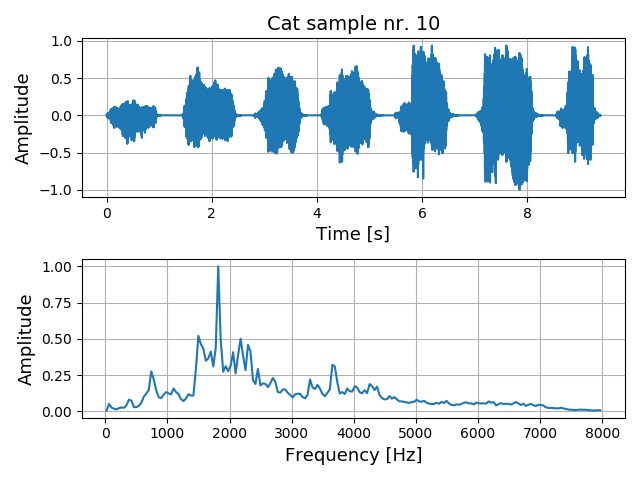
\includegraphics[scale=0.45]{../figures/cat_10_nbins200.png}
		\caption{Cat sample nr. 10}
	\end{subfigure}
	\begin{subfigure}{0.49\textwidth}
		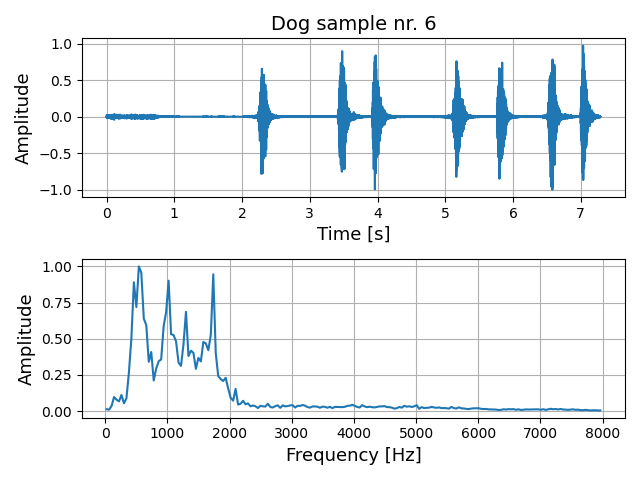
\includegraphics[scale=0.45]{../figures/dog_6_nbins200.png}
		\caption{Dog sample nr. 6}
	\end{subfigure}
	\caption{Time and frequency signal for one of the cat (left panel) samples, and one of the dog (right panel) samples. The amplitudes are normalized.}
	\label{fig:cat_dog_samples}
\end{figure}
We also use PCA to create a dimensionally reduced data set to test our classification methods with.
%We also use PCA decomposition of the data set to test our methods with. 
As the data set is fairly small, there is no problem using the full PCA, and we perform the reduction by keeping 95\% of the variance. This reduces our 200 frequency bins down to only 35 predictors, giving an 83\% reduction in the dimensionality of our data set.
%%%%%%%%%%%%%%%%%%%%%%%%%%%%%%%%%%%%%%%%%%%%%%%%%%%%%%%%%%%%%%%%%%%%%%%%%%%%%%%%%%%%%%%%%%
%%%%%%%%%%%%%%%%%%%%%%%%%%%%%%%%%%%%%%%%%%%%%%%%%%%%%%%%%%%%%%%%%%%%%%%%%%%%%%%%%%%%%%%%%%

\section{Results and discussion} \label{chap:results}
%\red{1. only best params, confusion matrix (+ roc/auc) in results. \\2. heatmaps and parameter combinations in appendices}
%\\\\
In this section we will go through the results from analyzing the data set described in Chapter \ref{chap:data_sets}, using different classification methods and dimensionality reduction. The code used to generate the results can be found in the GitHub repository \cite{Github3}, and is implemented using Scikit-Learn \cite{scikit-learn} in order to be able to parallelize the hyperparameter search\footnote{In the previous project \cite{Github2}, one of the grid searches took over 15 hours. Even though this data set is smaller, allowing the code to use more cores/threads (in the authors case, 12 threads) should reduce the run time significantly, allowing us to evaluate a larger part of the hyperparameter space.}. Cross-validation is employed during the hyperparameter search in order to more properly evaluate the results.
%\\\\
%\red{USE GRADIENT BOOSTING METHODS POTENTIALLY TO PENALIZE MISCLASSIFICATIONS MORE.}
\subsection{Neural networks}
We find our optimal hyperparameters for the neural net by performing grid search using the hyperparameter sets found in appendix \ref{app:nn_heatmaps}. For simplicity we set all hidden layers to have the same amount of nodes, however a more proper analysis would be useful. When trying the different solvers discussed earlier, it proved difficult to find any parameters where the stochastic gradient descent managed to converge properly. This was however not a problem with the quasi-Newton solver, so all the results presented here uses the \texttt{lbfgs} solver.
\subsubsection{Full data set}
Table \ref{tab:best_fit_nn_nonpca} shows our best-fit hyperparameters for the neural net. Some of the hyperparameter heatmaps can be found in appendix \ref{app:nn_heatmaps}, figure \ref{fig:app_nn_nonpca}. We note that the logistic function gives the best results, with tanh being the second best. In the previous project \cite{Github2}, we found that the ReLU activation performed the best for regression, and the worst for classification. Very curious is the fact that the best model is one with only one hidden layer, containing only one neuron. Looking at panel (d) in figure \ref{fig:app_nn_nonpca} we see how the results change depending on the depth and width of the neural network.
\begin{table}[H]
  \centering
  \caption{Best-fit hyperparameters for feed-forward neural network. Full data set.}
  \label{tab:best_fit_nn_nonpca}
  \begin{tabular}{c|c}
    \hline\hline
    Parameter & Value\\\hline
    n hidden neurons &  $1$\\
    n hidden layers &  $1$\\
    activation & logistic \\
    $\lambda$/$\alpha$  & $0.0001$\\
%    learning rate & $0.01$ \\
    max iterations & $600$
    \end{tabular}
\end{table}
Figure \ref{fig:nn_confusion_nonpca} shows the confusion matrix for the best-fit neural net, showing that the model performs quite a bit better at classifying the dog samples (96\%) compared to the cat samples (88\%). This gives us a total accuracy of $0.911$, which is still good.
\begin{figure}[H]
	\centering
	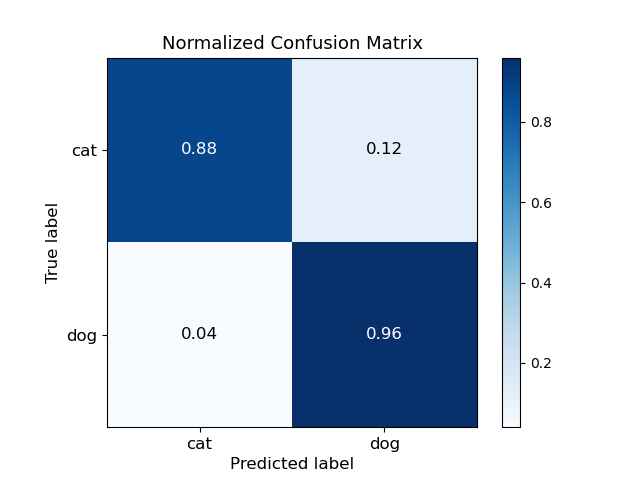
\includegraphics[scale=0.7]{../figures/neural_net/confusion_matrix_nbins200_pca0_seed4155_ts0.20.png}
	\caption{Confusion matrix for the neural net, full data set. The rows are normalized, showing the ratio of correctly/incorrectly labeled samples for each class.}
	\label{fig:nn_confusion_nonpca}
\end{figure}	
Figure \ref{fig:nn_roc_nonpca} shows the ROC curve for the best-fit neural net. We see that both of the class curves are good, with the same AUC score.
\begin{figure}[H]
	\centering
	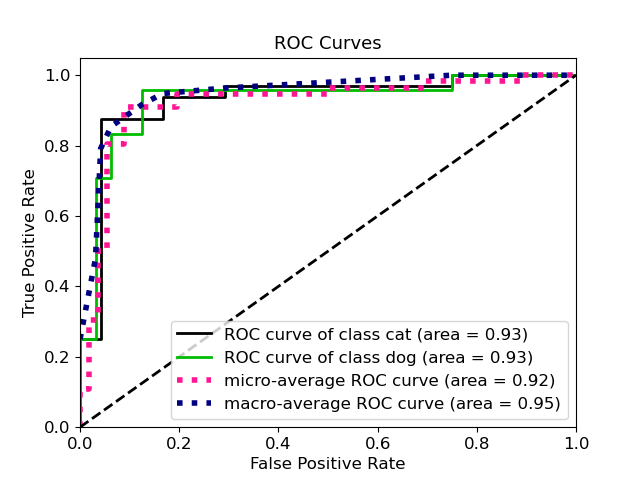
\includegraphics[scale=0.6]{../figures/neural_net/roc_nbins200_pca0_seed4155_ts0.20.png}
	\caption{ROC curve for the neural net, full data set. The AUC is given in the legend.}
	\label{fig:nn_roc_nonpca}
\end{figure}	

\subsubsection{PCA reduced data set}
For the PCA reduced data set, we run with the same hyperparameter sets as earlier, and get the following best-fit parameters, as shown in table \ref{tab:best_fit_nn_pca}. Some of the hyperparameter heatmaps can be seen in figure \ref{fig:app_nn_pca}. This time, a larger regularization strength is chosen, and we see that the best model contains a few more hidden neurons.
\begin{table}[H]
  \centering
  \caption{Best-fit hyperparameters for feed-forward neural network. PCA reduced data set.}
  \label{tab:best_fit_nn_pca}
  \begin{tabular}{c|c}
    \hline\hline
    Parameter & Value\\\hline
    n hidden neurons &  $5$\\
    n hidden layers &  $1$\\
    activation & logistic \\
    $\lambda$/$\alpha$  & $0.1$\\
%    learning rate & $0.01$ \\
    max iterations & $400$
    \end{tabular}
\end{table}
Training our neural net with the best-fit parameters we get the following confusion matrix for the PCA reduced data set, shown in figure \ref{fig:nn_confusion_pca}. Here, we see that the true positives remain the same (maybe slight improvement as blue color is a bit darker), while the model loses 4\% at classifying dogs. This could be due to the larger probable variation in frequencies used by dogs of different sizes, and thus when reducing the dimensions, the information lost affects dogs more. The disparity in sample sizes for both classes could also affect this to some extent.
\begin{figure}[H]
	\centering
	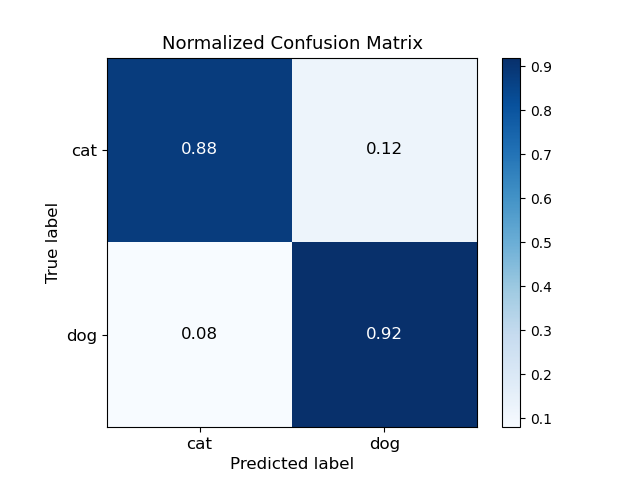
\includegraphics[scale=0.7]{../figures/neural_net/confusion_matrix_nbins200_pca35_seed4155_ts0.20.png}
	\caption{Confusion matrix for the neural net, PCA reduced data set. The rows are normalized, showing the ratio of correctly/incorrectly labeled samples for each class.}
	\label{fig:nn_confusion_pca}
\end{figure}	
Figure \ref{fig:nn_roc_pca} shows the ROC curves for the best-fit neural net. Similar to the full data set, it is hard to tell anything beyond that the models seem to perform well. The AUC is slightly higher than before though, despite the total accuracy for the model decreasing slightly.
\begin{figure}[H]
	\centering
	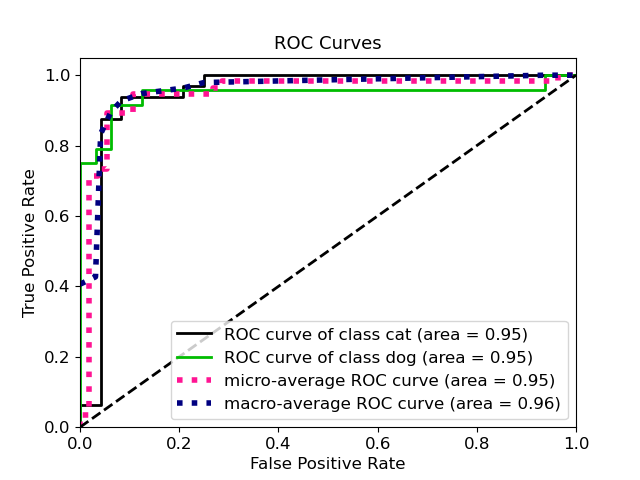
\includegraphics[scale=0.6]{../figures/neural_net/roc_nbins200_pca35_seed4155_ts0.20.png}
	\caption{ROC curve for the neural net, PCA reduced data set. The AUC is given in the legend.}
	\label{fig:nn_roc_pca}
\end{figure}	

\subsection{Random forests}
We find our optimal hyperparameters for random forests by performing grid search using the hyperparameter sets found in appendix \ref{app:rf_heatmaps}.
\subsubsection{Full data set}
Table \ref{tab:best_fit_rf_nonpca} shows our best-fit hyperparameters for random forests. Some of the hyperparameter heatmaps can be found in appendix \ref{app:rf_heatmaps}, figure \ref{fig:app_rf_nonpca}.
\begin{table}[H]
  \centering
  \caption{Best-fit hyperparameters for random forests. Full data set.}
  \label{tab:best_fit_rf_nonpca}
  \begin{tabular}{c|c}
    \hline\hline
    Parameter & Value\\\hline
    n estimators &  $15$\\
    max depth &  $7$\\
    min samples split & $2$ \\
    min samples leaf  & $5$\\
    max features & $7$ %\\
%    max leaf nodes & $0.1$
    \end{tabular}
\end{table}
Figure \ref{fig:rf_confusion_nonpca} shows the confusion matrix for the best-fit random forest. Here, the results are almost inverse of what was found for the neural net. The random forest performs extremely well at classifying cat samples, at 97\% accuracy, while dogs end up with only 83\%. This cat accuracy comes at the cost of dogs, leading our model to guess dogs more often, as seen in the false negatives.
\begin{figure}[H]
	\centering
	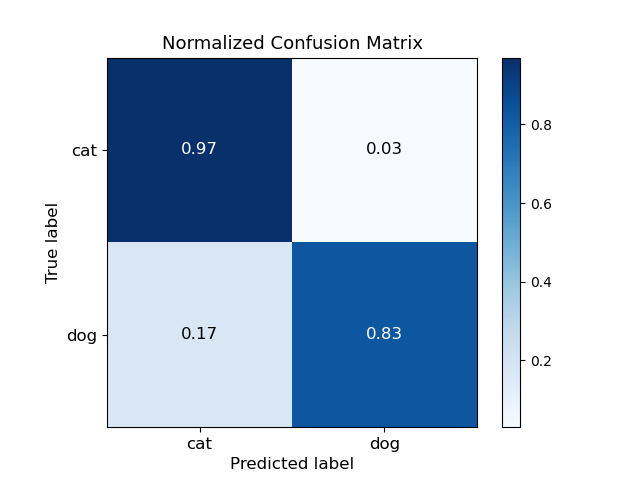
\includegraphics[scale=0.7]{../figures/random_forest/confusion_matrix_nbins200_pca0_seed4155_ts0.20.png}
	\caption{Confusion matrix for random forests, full data set. The rows are normalized, showing the ratio of correctly/incorrectly labeled samples for each class.}
	\label{fig:rf_confusion_nonpca}
\end{figure}	
Figure \ref{fig:rf_roc_nonpca} shows the ROC curve for the random forest. The AUC is the same for both classes, so either something is wrong with our implementation, or it really is as mentioned earlier quite problematic for evaluating model fit.
\begin{figure}[H]
	\centering
	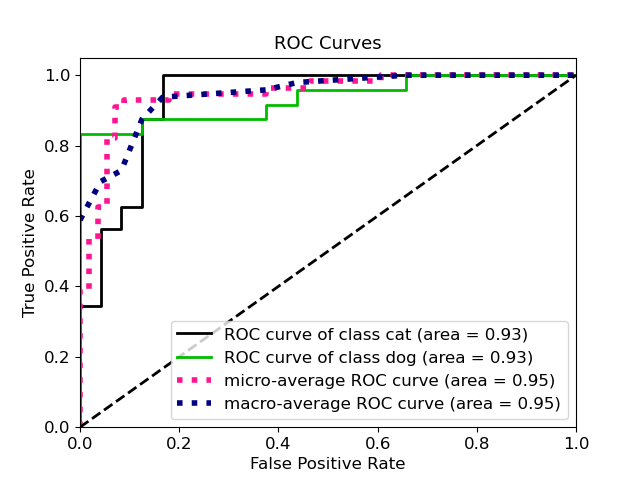
\includegraphics[scale=0.6]{../figures/random_forest/roc_nbins200_pca0_seed4155_ts0.20.png}
	\caption{ROC curve for random forests, full data set. The AUC is given in the legend.}
	\label{fig:rf_roc_nonpca}
\end{figure}	

\subsubsection{PCA reduced data set}
Table \ref{tab:best_fit_rf_pca} shows our best-fit hyperparameters for the PCA reduced data set. Some of the hyperparameter heatmaps can be found in appendix \ref{app:rf_heatmaps}, figure \ref{fig:app_rf_pca}. We note that compared to the full data set, there is a higher amount of trees made. The trees are less deep (max depth 3 vs 7), however a higher amount of features is considered for each tree, which along with the fact that there are less features in total, means that $37$\% of all dimensions are considered for each tree, compared to $3.5$\% for the full set.

\begin{table}[H]
  \centering
  \caption{Best-fit hyperparameters for random forests. PCA reduced data set.}
  \label{tab:best_fit_rf_pca}
  \begin{tabular}{c|c}
    \hline\hline
    Parameter & Value\\\hline
    n estimators &  $25$\\
    max depth &  $3$\\
    min samples split & $2$ \\
    min samples leaf  & $8$\\
    max features & $13$ %\\
%    max leaf nodes & $0.1$
    \end{tabular}
\end{table}
Figure \ref{fig:rf_confusion_pca} shows the confusion matrix for the random forest with the PCA reduced data set. We see that the predictive power drops for the cat class, however the dog accuracy increases. Similar to the full data set, the results are the opposite of the equivalent neural net result, with the random forest being better at classifying the cat samples rather than dogs.
\begin{figure}[H]
	\centering
	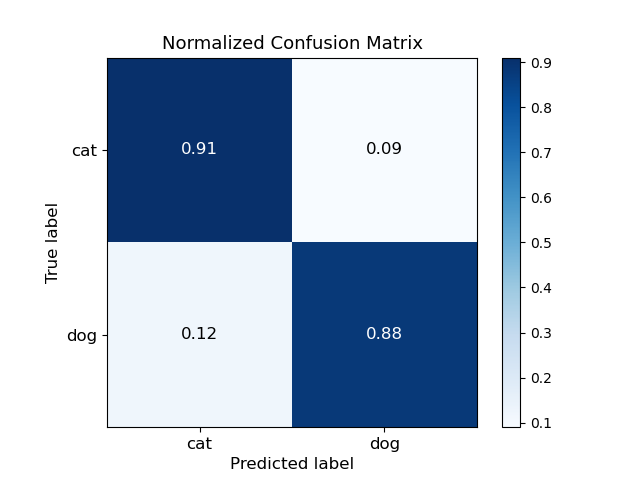
\includegraphics[scale=0.7]{../figures/random_forest/confusion_matrix_nbins200_pca35_seed4155_ts0.20.png}
	\caption{Confusion matrix for random forests, PCA reduced data set. The rows are normalized, showing the ratio of correctly/incorrectly labeled samples for each class.}
	\label{fig:rf_confusion_pca}
\end{figure}	
Figure \ref{fig:rf_roc_pca} shows the ROC curves for the PCA reduced data set. Here, the curves for both classes are very close to each other, which kinda makes sense given the similar accuracy seen in the confusion matrix. The AUC however is higher than it was for the full data set.
\begin{figure}[H]
	\centering
	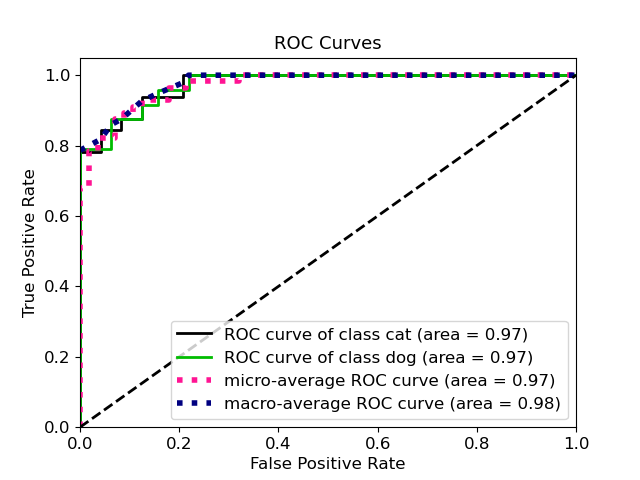
\includegraphics[scale=0.6]{../figures/random_forest/roc_nbins200_pca35_seed4155_ts0.20.png}
	\caption{ROC curve for random forests, PCA reduced data set. The AUC is given in the legend.}
	\label{fig:rf_roc_pca}
\end{figure}	


\subsection{XGBoost}
Finally, we move on to XGBoost, and find our optimal hyperparameters by performing grid search using the hyperparameter sets found in appendix \ref{app:xgboost_heatmaps}.

\subsubsection{Full data set}
Table \ref{tab:best_fit_xgboost_nonpca} shows our best-fit hyperparameters for XGBoost. Some of the hyperparameter heatmaps can be found in appendix \ref{app:xgboost_heatmaps}, figure \ref{fig:app_xgboost_nonpca}. We see that no regularization is preferred. Testing a larger set of learning rates might have been useful.
\begin{table}[H]
  \centering
  \caption{Best-fit hyperparameters for XGBoost. Full data set.}
  \label{tab:best_fit_xgboost_nonpca}
  \begin{tabular}{c|c}
    \hline\hline
    Parameter & Value\\\hline
    learning rate  & $0.2$\\
    n estimators &  $100$\\
    max depth &  $4$\\
    min child weight & $7$ \\
    lambda & $0.0$
    \end{tabular}
\end{table}
From the best-fit hyperparameters, we get the following confusion matrix for XGBoost, shown in figure \ref{fig:xgboost_confusion_nonpca}. We see that XGBoost performs extremely well for both classes, with a ~95\% accuracy for both classes combined. Like with random forests, XGBoost performs better at classifying cat samples.
\begin{figure}[H]
	\centering
	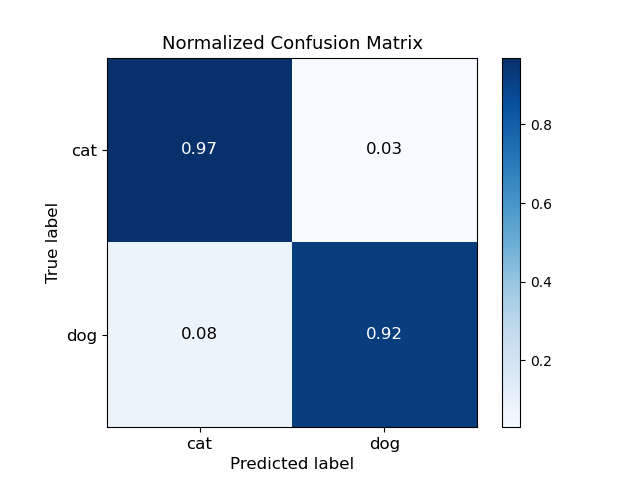
\includegraphics[scale=0.7]{../figures/xgboost/confusion_matrix_nbins200_pca0_seed4155_ts0.20.png}
	\caption{Confusion matrix for XGBoost, full data set. The rows are normalized, showing the ratio of correctly/incorrectly labeled samples for each class.}
	\label{fig:xgboost_confusion_nonpca}
\end{figure}
Figure \ref{fig:xgboost_roc_nonpca} shows the ROC curves and AUC score for XGBoost. Like previously, it is hard to gauge anything useful from the plot, beyond it performing well.
\begin{figure}[H]
	\centering
	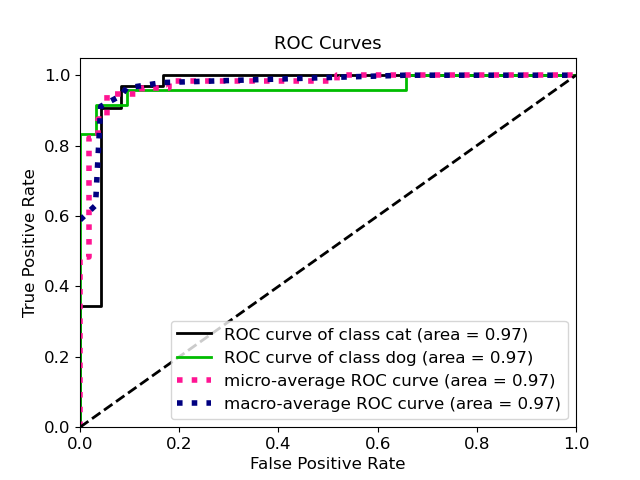
\includegraphics[scale=0.6]{../figures/xgboost/roc_nbins200_pca0_seed4155_ts0.20.png}
	\caption{ROC curve for XGBoost, full data set. The AUC is given in the legend.}
	\label{fig:xgboost_roc_nonpca}
\end{figure}	

\subsubsection{PCA reduced data set}
Table \ref{tab:best_fit_xgboost_pca} shows our best-fit hyperparameters for XGBoost with the PCA reduced data set. Some of the hyperparameter heatmaps can be found in appendix \ref{app:xgboost_heatmaps}, figure \ref{fig:app_xgboost_pca}. We note that a smaller set of shallower trees is preferred, with the amount of estimators almost matching the reduction in dimensionality.

\begin{table}[H]
  \centering
  \caption{Best-fit hyperparameters for XGBoost. PCA reduced data set.}
  \label{tab:best_fit_xgboost_pca}
  \begin{tabular}{c|c}
    \hline\hline
    Parameter & Value\\\hline
    learning rate  & $0.3$\\
    n estimators &  $20$\\
    max depth &  $2$\\
    min child weight & $1$ \\
    lambda & $0.0$
    \end{tabular}
\end{table}
Figure \ref{fig:xgboost_confusion_pca} shows the confusion matrix with XGBoost on the PCA reduced data set. The correctly guessed cat samples decreases by 3 percentage points, while the dog accuracy remains unchanged. The total accuracy drops slightly, but it still outperforms the neural net and random forests.

\begin{figure}[H]
	\centering
	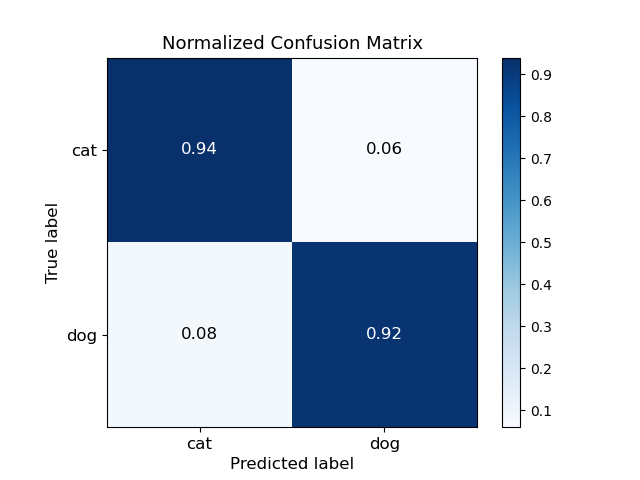
\includegraphics[scale=0.7]{../figures/xgboost/confusion_matrix_nbins200_pca35_seed4155_ts0.20.png}
	\caption{Confusion matrix for XGBoost, PCA reduced data set. The rows are normalized, showing the ratio of correctly/incorrectly labeled samples for each class.}
	\label{fig:xgboost_confusion_pca}
\end{figure}	
Figure \ref{fig:xgboost_roc_pca} shows the ROC curves and AUC score for the PCA reduced data set. Like with neural net and random forests, the ROC curves and AUC scores seem to be better for the dimensionality reduced data set, despite the model accuracy being lower in all cases.

\begin{figure}[H]
	\centering
	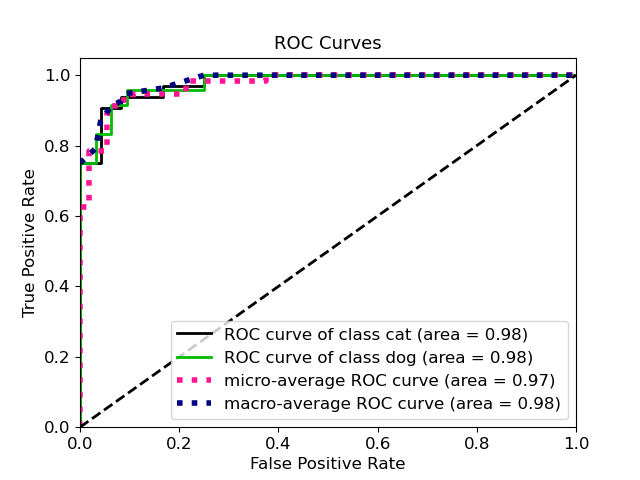
\includegraphics[scale=0.6]{../figures/xgboost/roc_nbins200_pca35_seed4155_ts0.20.png}
	\caption{ROC curve for XGBoost, PCA reduced data set. The AUC is given in the legend.}
	\label{fig:xgboost_roc_pca}
\end{figure}	

\subsection{Time}
Table \ref{tab:timing} shows the average time the training/fit process took for each of the three classification methods, for both versions of the data set. We see that for the full data set, random forest is the fastest method, being roughly 3 times as fast for training compared to XGBoost. Since we used the parameter setting for number of decision trees for both of them, that is not the reason for the discrepancy either. The neural net on the other hand was extremely slow.
\\\\
When using the PCA reduced data set both the neural net and XGBoost decreased their run time by a decent amount. This data set has roughly 1/6th as many dimensions as the full one, with neural net speeding up by 2.25 times, and XGBoost at 4.03 times faster, so the run times don't scale linearly with predictor size. Curiously enough, the random forest training time does not change.

%\red{LBFGS is fast, SGD is not, took ~420 ms on average.} 
\begin{table}[H]
  \centering
  \caption{Average fit/training time for the three different methods examined, given in milliseconds for both the full dimensional data set and the PCA reduced data set.}
  \label{tab:timing}
  \begin{tabular}{c|c|c}
    \hline\hline
    Method & Time full data set [$ms$] & Time reduced data set [$ms$] \\\hline
%    Neural net (adam) & 235.0 & 177.0 \\
    Neural net & $732$ & $325$ \\
    Random forest & $28.4$ & $28.3$ \\
    XGBoost & $83.9$ & $20.8$
    \end{tabular}
\end{table}
As the parameter grid search has been run in parallel on all CPU threads, this test does end up somewhat depending on computer load, and while we attempted to limit other things running at the same time, its hard to say exactly how accurate they are, beyond the fact that neural nets were significantly slower.

\subsection{Summary of results}
The results are summarized in table \ref{tab:summary}, showing the total accuracy and the ROC AUC for each of the three methods. We see that neural nets and random forests perform the same when looking at the accuracy, however there is a small improvement with the AUC when using the PCA reduced data set. Given the runtime differences between FFNN and RF mentioned earlier, and the convergence issues, random forest is the best option of the two. XGBoost performs better than both of them however, performing at over 90\% for both data set versions.
\begin{table}[H]
  \centering
  \caption{Summary of the accuracy and AUC scores for each of the classification methods. The AUC score corresponds to the micro-average found in the ROC plots. The micro-average is used as there is a class imbalance due to there being more cat samples than dogs.}
  \label{tab:summary}
  \begin{tabular}{c|c|c||c|c}
    \hline\hline
    Method & Accuracy & ROC AUC & Accuracy (PCA) & ROC AUC (PCA) \\\hline
    Neural net & $0.911$ & $0.92$ & $0.893$ & $0.95$ \\
    Random forest & $0.911$ & $0.95$ & $0.893$ & $0.97$ \\
    XGBoost & $0.946$ & $0.97$ & $0.929$ & $0.97$
    \end{tabular}
\end{table}

%%%%%%%%%%%%%%%%%%%%%%%%%%%%%%%%%%%%%%%%%%%%%%%%%%%%%%%%%%%%%%%%%%%%%%%%%%%%%%%%%%%%%%%%%%
%%%%%%%%%%%%%%%%%%%%%%%%%%%%%%%%%%%%%%%%%%%%%%%%%%%%%%%%%%%%%%%%%%%%%%%%%%%%%%%%%%%%%%%%%%
\section{Conclusion} \label{chap:conclusion}
In this project, we set out to investigate how a frequency-space approach to classifying different animal sounds performs when using feed-forward neural nets, random forests, and the gradient boosting method XGBoost. The data set was a set of audio files containing cat and dog sounds, that were transformed into frequency space using Fourier transform, and then binned into 40 Hz bins. We also tested PCA to see if further reducing the amount of dimensions yielded improvements to either accuracy or run time.
\\\\
%\red{results}
For the full data set we find that both the feed-forward neural net and the random forest performs exactly the same, with an accuracy of 91\%. Random forest has a slightly better AUC score, however all ROC/AUC results seem odd. XGBoost performs even better than both of them with an accuracy of almost 95\%.
\\\\
For the PCA reduced data set, very similar differences were found, with everything shifted downwards accuracy wise. Neural nets and random forests got an accuracy score of 89\%, while XGBoost also here performed the best with an accuracy of 93\%.
\\\\
For both data sets, FFNN classified dogs better than cats, while RF and XGBoost classified cats more accurately than dogs. The difference between the classes decreased however with the PCA reduced data set for all methods. Time wise, FFNN was by far the slowest, while RF was faster than XGBoost for the full data set. For the reduced data set, XGBoost was the fastest, while RF remained unchanged.
%In this project, we set out to investigate how stochastic gradient descent and feed-forward neural networks work on both regression and classification problems. We used cross-validation in order to assess which of the hyperparameter combinations gave the best fit.
%\\\\
%For the Franke function, we found that both SGD and FFNN performed worse than OLS and Ridge, though the neural net got much closer, with an $R^2$ score of $0.93$, while SGD got $0.84$, none of which are bad. For both, we found that the largest number of epochs $\Nepochs = 100$ and the largest learning rate $\eta=0.1$ gave the best results. SGD preferred a batch size of 5, with no regularization for $p=8$, and $\lambda=0.001$ at $p=15$, showing similar behavior with how OLS and Ridge performed for those polynomial degrees. The neural net yielded much better results as the batch size is increased. Based on tests, it seems that using either one of the ReLu family activation functions would have improved the results.
%\\\\
%For the classification case, where we studied a reduced version of the MNIST data set, both the SGD and Neural net performed exceedingly well, outperforming the equivalent Scikit-Learn implementation. The SGD implementation gave an accuracy of 96\%, which starts to approach what you would expect from human accuracy. SKL was within a percent point away from it. The NN code yielded an accuracy of 95\%, but doing so with only 10 epochs and 10 nodes in the singular hidden layer. 
\\\\
For future work it would have been interesting to create an ensemble method consisting of neural nets and either of the other methods, as the former was better at classifying dogs, while random forests and XGBoost performed better when classifying cats, so this might lead us to an even better performing classifier. A closer look at the frequency spectra for the misclassified samples might have yielded some insight into the classification differences. It might also be beneficial to use something else than grid search in order to find better hyperparameters. Finally, it would be interesting to see how well our method performs on the full data set that \cite{Takahashi+2016} used, as it contained more classes than just the two used here.
%In hindsight, it might also be a good idea to let the model predict the probability that it is either a cat or a dog, making the output a one-hot vector instead of coding cat=0 and dog=1 as our targets.
%\red{Future, look at data with more classes, like the original set.}
%\red{FUTURE, LOOK AT RANDOM SEARCH FOR PARAMETERS INSTEAD OF grid saercarh}
%\red{Future, maybe combine results into an ensemble method as NN appeared to be better at classifying dogs, so this might give even better results. Both RF and XGBoost are better at classifying cats than dogs.}
%%%%%%%%%%%%%%%%%%%%%%%%%%%%%%%%%%%%%%%%%%%%%%%%%%%%%%%%%%%%%%%%%%%%%%%%%%%%%%%%%%%%%%%%%%
%%%%%%%%%%%%%%%%%%%%%%%%%%%%%%%%%%%%%%%%%%%%%%%%%%%%%%%%%%%%%%%%%%%%%%%%%%%%%%%%%%%%%%%%%%
\bibliography{references}
%%%%%%%%%%%%%%%%%%%%%%%%%%%%%%%%%%%%%%%%%%%%%%%%%%%%%%%%%%%%%%%%%%%%%%%%%%%%%%%%%%%%%%%%%%
%%%%%%%%%%%%%%%%%%%%%%%%%%%%%%%%%%%%%%%%%%%%%%%%%%%%%%%%%%%%%%%%%%%%%%%%%%%%%%%%%%%%%%%%%%

\appendix
\section*{Appendix} \label{chap:appendix}
%\section{Appendix} \label{chap:appendix}

\section{Neural Net Heatmaps} \label{app:nn_heatmaps}
The following hyperparameter sets were used for finding best fit parameters as well as heatmaps below.
\begin{align*}
	\text{n hidden neurons} &\in \{1, 5, 10, 25, 50, 75, 100\}\\
	\text{n hidden layers} &\in \{1, 2, 3, 4, 5\}\\
	\text{max iterations} &\in \{200, 300, 400, 500, 600\}\\
	\text{activation} &\in \{\text{relu}, \text{logistic}, \text{tanh}, \text{identity}\}\\
	\text{lambda} &\in \{0.1, 0.01, 0.001, 0.0001, 0.0\}
%	\text{batch size} &\in \{1, 5, 10, 50\}\\
%	\eta_0 &\in \{0.1, 0.01, 0.001\}\\
\end{align*}

\subsection{Without PCA}
\begin{figure}[H]
  \centering
  \begin{subfigure}{0.49\textwidth}
    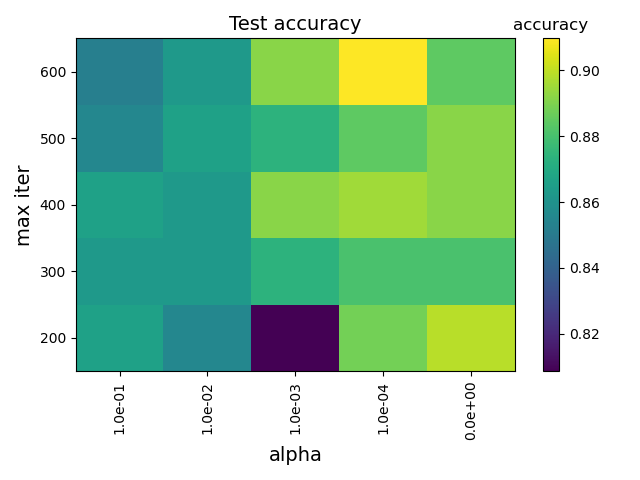
\includegraphics[scale=0.45]{../figures/neural_net/heatmaps/heatmap_nbins200_pca0_seed4155_ts0.20_accuracy_alpha_max_iter.png}
    \caption{Regularization vs maximum iterations}
  \end{subfigure}
  \begin{subfigure}{0.49\textwidth}
    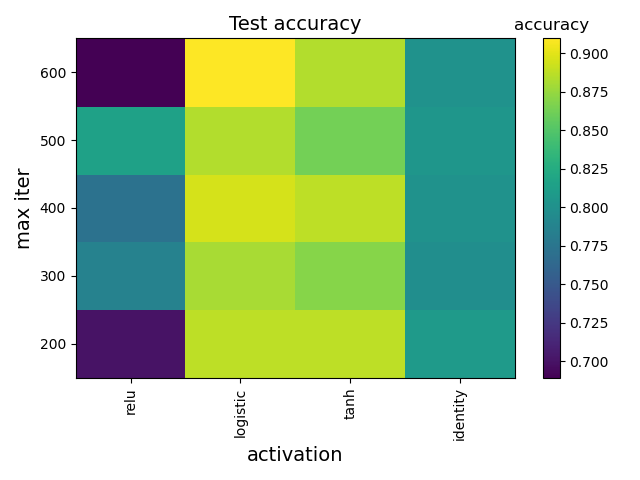
\includegraphics[scale=0.45]{../figures/neural_net/heatmaps/heatmap_nbins200_pca0_seed4155_ts0.20_accuracy_activation_max_iter.png}
    \caption{Activation function vs maximum iterations}
  \end{subfigure}\\
  \begin{subfigure}{0.49\textwidth}
    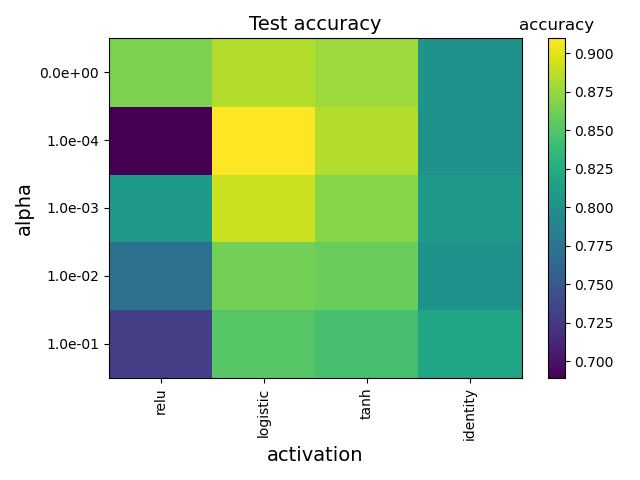
\includegraphics[scale=0.45]{../figures/neural_net/heatmaps/heatmap_nbins200_pca0_seed4155_ts0.20_accuracy_activation_alpha.png}
    \caption{Activation function vs regularization}
  \end{subfigure}
  \begin{subfigure}{0.49\textwidth}
    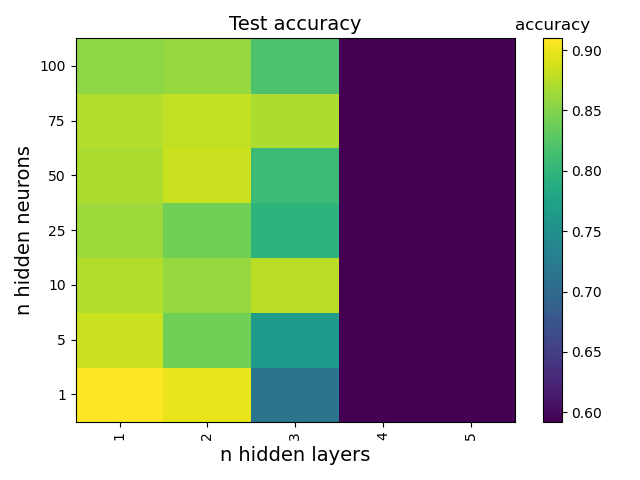
\includegraphics[scale=0.45]{../figures/neural_net/heatmaps/heatmap_nbins200_pca0_seed4155_ts0.20_accuracy_n_hidden_layers_n_hidden_neurons.png}
    \caption{Number of layers vs number of hidden neurons}
  \end{subfigure}
  \caption{Accuracy heatmaps for different hyperparameters. Neural net, full data set. All other hyperparameters set to the best-fit from table \ref{tab:best_fit_nn_nonpca}.}
  \label{fig:app_nn_nonpca}
\end{figure}

\subsection{With PCA}

\begin{figure}[H]
  \centering
  \begin{subfigure}{0.49\textwidth}
    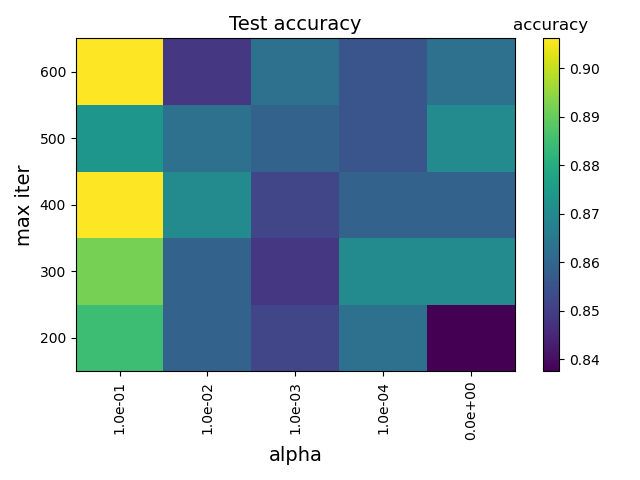
\includegraphics[scale=0.45]{../figures/neural_net/heatmaps/heatmap_nbins200_pca35_seed4155_ts0.20_accuracy_alpha_max_iter.png}
    \caption{Regularization vs maximum iterations}
  \end{subfigure}
  \begin{subfigure}{0.49\textwidth}
    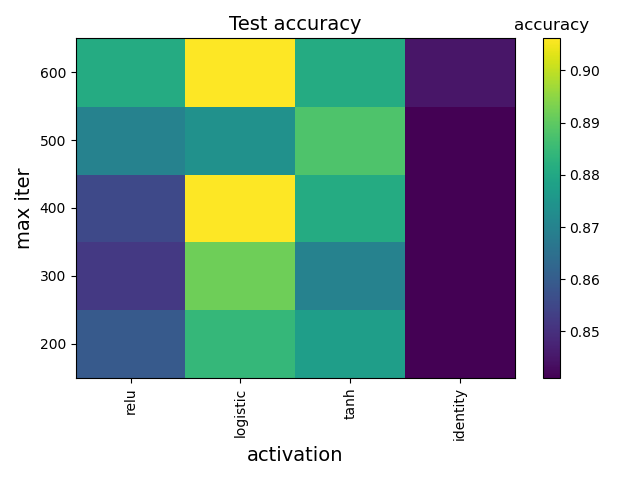
\includegraphics[scale=0.45]{../figures/neural_net/heatmaps/heatmap_nbins200_pca35_seed4155_ts0.20_accuracy_activation_max_iter.png}
    \caption{Activation function vs maximum iterations}
  \end{subfigure}\\
  \begin{subfigure}{0.49\textwidth}
    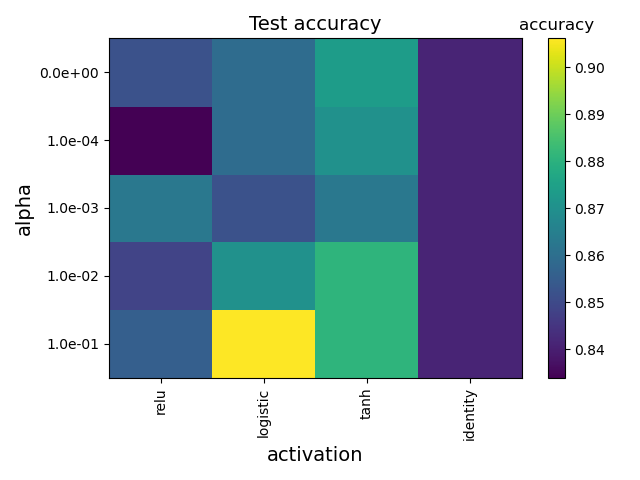
\includegraphics[scale=0.45]{../figures/neural_net/heatmaps/heatmap_nbins200_pca35_seed4155_ts0.20_accuracy_activation_alpha.png}
    \caption{Activation function vs regularization}
  \end{subfigure}
  \begin{subfigure}{0.49\textwidth}
    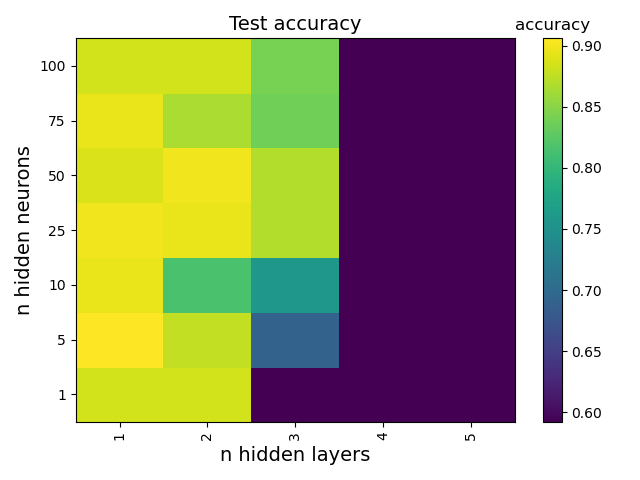
\includegraphics[scale=0.45]{../figures/neural_net/heatmaps/heatmap_nbins200_pca35_seed4155_ts0.20_accuracy_n_hidden_layers_n_hidden_neurons.png}
    \caption{Number of layers vs number of hidden neurons}
  \end{subfigure}
  \caption{Accuracy heatmaps for different hyperparameters. Neural net, reduced data set. All other hyperparameters set to the best-fit from table \ref{tab:best_fit_nn_pca}.}
  \label{fig:app_nn_pca}
\end{figure}


%%%%%%%%%%%%%%%%%%%%%%%%%%%%%%%%%%%%%%%%%%%%%%%%%%%%%%%%%%%%%%%%%%%%%%%%%%%%%%%%%%%%%%%%%%
%%%%%%%%%%%%%%%%%%%%%%%%%%%%%%%%%%%%%%%%%%%%%%%%%%%%%%%%%%%%%%%%%%%%%%%%%%%%%%%%%%%%%%%%%%

\section{Random Forests Heatmaps} \label{app:rf_heatmaps}
The following hyperparameter sets were used for finding best fit parameters as well as heatmaps below.
\begin{align*}
	\text{max depth} &\in \{3, 5, 7, 9, 12\}\\
	\text{max features} &\in \{3, 5, 7, 10, 13\}\\
	\text{min samples leaf} &\in \{5, 8, 10, 12\}\\
	\text{min samples split} &\in \{2, 3, 4, 5, 7, 9\}\\
	\text{n estimators} &\in \{2, 5, 7, 10, 15, 25, 50, 100\}
\end{align*}

\subsection{Without PCA}

\begin{figure}[H]
  \centering
  \begin{subfigure}{0.49\textwidth}
    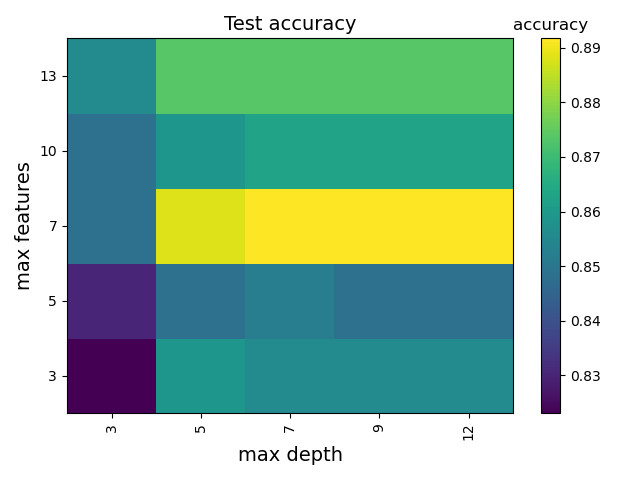
\includegraphics[scale=0.45]{../figures/random_forest/heatmaps/heatmap_nbins200_pca0_seed4155_ts0.20_accuracy_max_depth_max_features.png}
    \caption{Max depth vs max features}
  \end{subfigure}
  \begin{subfigure}{0.49\textwidth}
    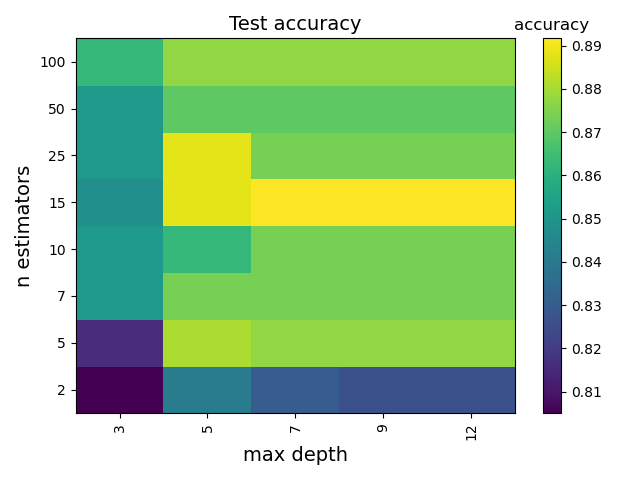
\includegraphics[scale=0.45]{../figures/random_forest/heatmaps/heatmap_nbins200_pca0_seed4155_ts0.20_accuracy_max_depth_n_estimators.png}
    \caption{Max depth vs n estimators}
  \end{subfigure}\\
  \begin{subfigure}{0.49\textwidth}
    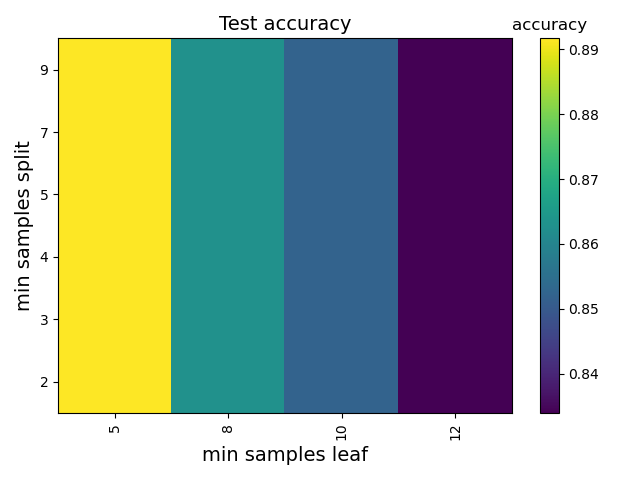
\includegraphics[scale=0.45]{../figures/random_forest/heatmaps/heatmap_nbins200_pca0_seed4155_ts0.20_accuracy_min_samples_leaf_min_samples_split.png}
    \caption{Min samples leaf vs min samples split}
  \end{subfigure}
  \begin{subfigure}{0.49\textwidth}
    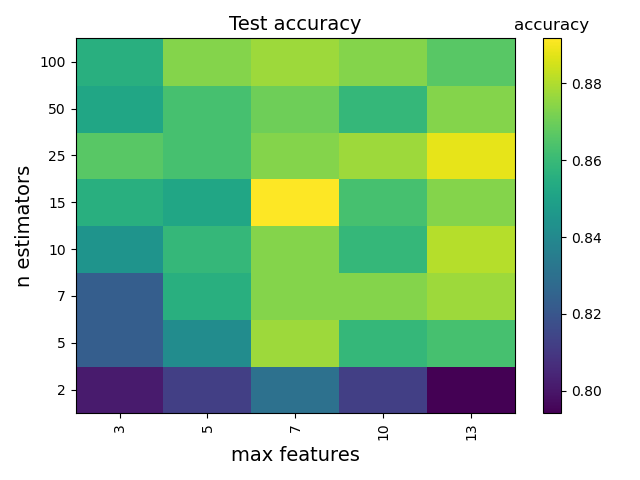
\includegraphics[scale=0.45]{../figures/random_forest/heatmaps/heatmap_nbins200_pca0_seed4155_ts0.20_accuracy_max_features_n_estimators.png}
    \caption{Max features vs n estimators}
  \end{subfigure}
  \caption{Accuracy heatmaps for different hyperparameters. Random forest, full data set. All other hyperparameters set to the best-fit from table \ref{tab:best_fit_rf_nonpca}.}
  \label{fig:app_rf_nonpca}
\end{figure}

\subsection{With PCA}

\begin{figure}[H]
  \centering
  \begin{subfigure}{0.49\textwidth}
    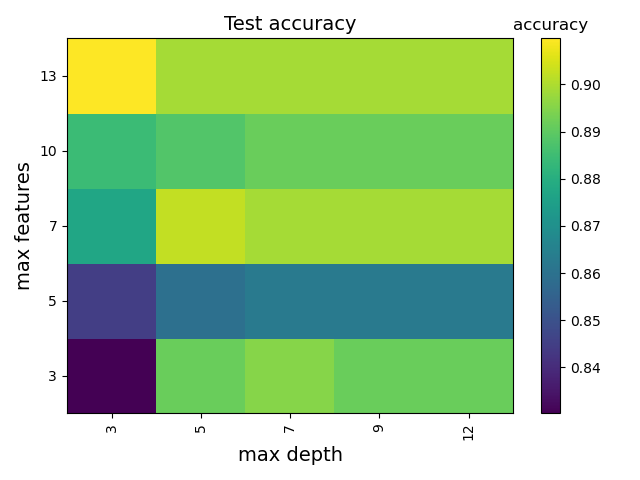
\includegraphics[scale=0.45]{../figures/random_forest/heatmaps/heatmap_nbins200_pca35_seed4155_ts0.20_accuracy_max_depth_max_features.png}
    \caption{Max depth vs max features}
  \end{subfigure}
  \begin{subfigure}{0.49\textwidth}
    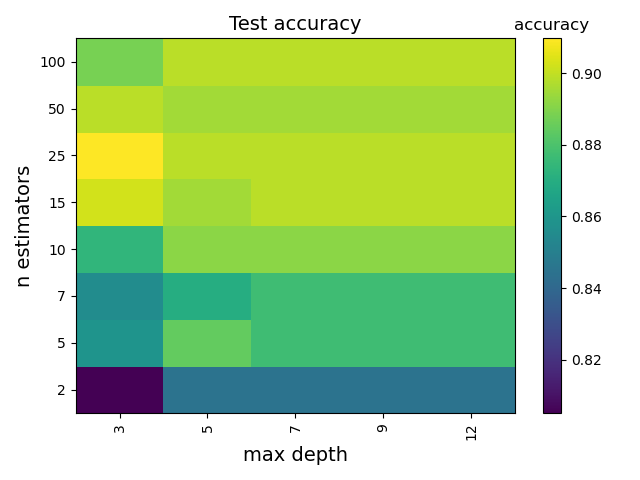
\includegraphics[scale=0.45]{../figures/random_forest/heatmaps/heatmap_nbins200_pca35_seed4155_ts0.20_accuracy_max_depth_n_estimators.png}
    \caption{Max depth vs n estimators}
  \end{subfigure}\\
  \begin{subfigure}{0.49\textwidth}
    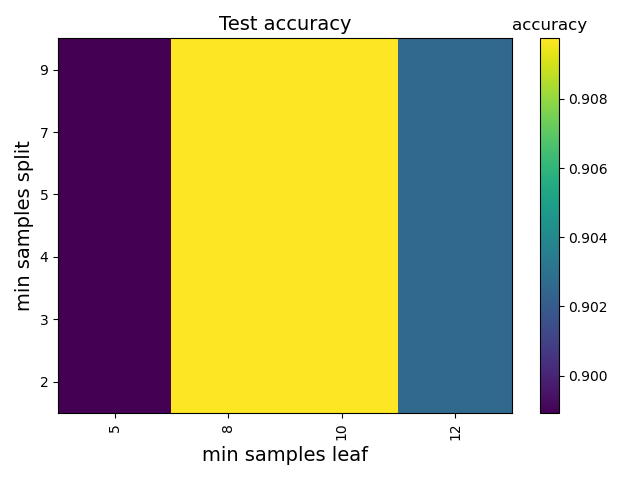
\includegraphics[scale=0.45]{../figures/random_forest/heatmaps/heatmap_nbins200_pca35_seed4155_ts0.20_accuracy_min_samples_leaf_min_samples_split.png}
    \caption{Min samples leaf vs min samples split}
  \end{subfigure}
  \begin{subfigure}{0.49\textwidth}
    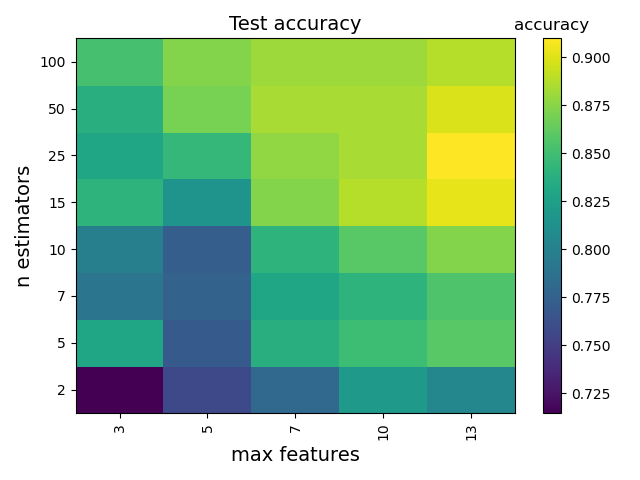
\includegraphics[scale=0.45]{../figures/random_forest/heatmaps/heatmap_nbins200_pca35_seed4155_ts0.20_accuracy_max_features_n_estimators.png}
    \caption{Max features vs n estimators}
  \end{subfigure}
  \caption{Accuracy heatmaps for different hyperparameters. Random forest, reduced data set. All other hyperparameters set to the best-fit from table \ref{tab:best_fit_rf_pca}.}
  \label{fig:app_rf_pca}
\end{figure}

%%%%%%%%%%%%%%%%%%%%%%%%%%%%%%%%%%%%%%%%%%%%%%%%%%%%%%%%%%%%%%%%%%%%%%%%%%%%%%%%%%%%%%%%%%
%%%%%%%%%%%%%%%%%%%%%%%%%%%%%%%%%%%%%%%%%%%%%%%%%%%%%%%%%%%%%%%%%%%%%%%%%%%%%%%%%%%%%%%%%%

\section{XGBoost Heatmaps} \label{app:xgboost_heatmaps}
The following hyperparameter sets were used for finding best fit parameters as well as heatmaps below.
\begin{align*}
	\text{learning rate} &\in \{0.05, 0.1, 0.2, 0.3\}\\
	\text{n estimators} &\in \{5, 10, 15, 20, 25, 50, 100\}\\
	\text{max depth} &\in \{2, 3, 4, 5, 6, 7, 8\}\\
	\text{min child weight} &\in \{1, 3, 5, 7, 10\}\\
	\text{lambda} &\in \{0.0, 0.1, 0.01, 0.001\}
\end{align*}

\subsection{Without PCA}

\begin{figure}[H]
  \centering
  \begin{subfigure}{0.49\textwidth}
    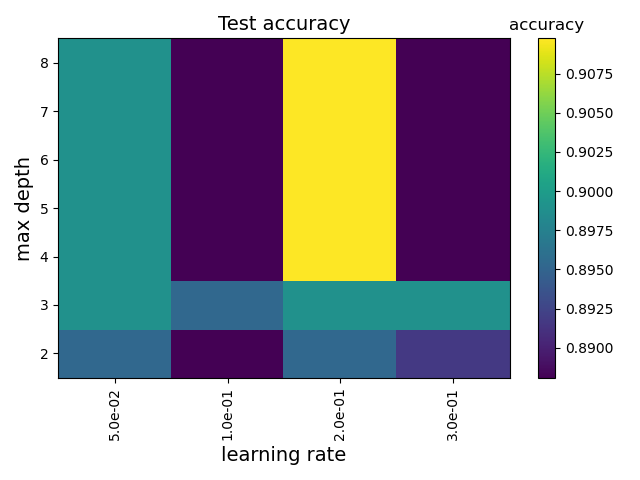
\includegraphics[scale=0.45]{../figures/xgboost/heatmaps/heatmap_nbins200_pca0_seed4155_ts0.20_accuracy_learning_rate_max_depth.png}
    \caption{Learning rate vs max depth}
  \end{subfigure}
  \begin{subfigure}{0.49\textwidth}
    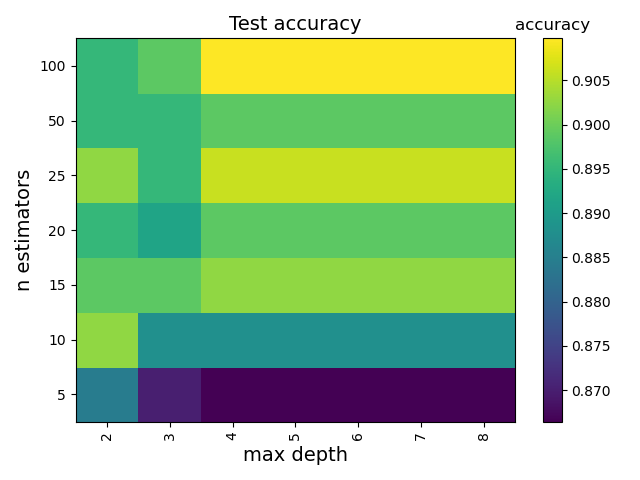
\includegraphics[scale=0.45]{../figures/xgboost/heatmaps/heatmap_nbins200_pca0_seed4155_ts0.20_accuracy_max_depth_n_estimators.png}
    \caption{Max depth vs n estimators}
  \end{subfigure}\\
  \begin{subfigure}{0.49\textwidth}
    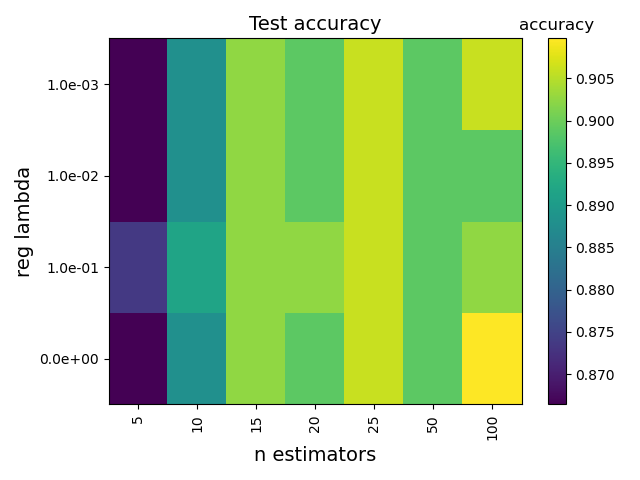
\includegraphics[scale=0.45]{../figures/xgboost/heatmaps/heatmap_nbins200_pca0_seed4155_ts0.20_accuracy_n_estimators_reg_lambda.png}
    \caption{Regularization vs n estimators}
  \end{subfigure}
  \begin{subfigure}{0.49\textwidth}
    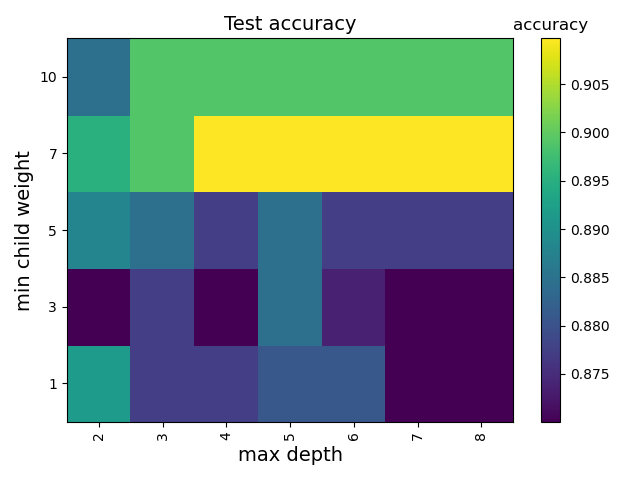
\includegraphics[scale=0.45]{../figures/xgboost/heatmaps/heatmap_nbins200_pca0_seed4155_ts0.20_accuracy_max_depth_min_child_weight.png}
    \caption{Max depth vs min child weight}
  \end{subfigure}
  \caption{Accuracy heatmaps for different hyperparameters. XGBoost, full data set. All other hyperparameters set to the best-fit from table \ref{tab:best_fit_xgboost_nonpca}.}
  \label{fig:app_xgboost_nonpca}
\end{figure}

\subsection{With PCA}

\begin{figure}[H]
  \centering
  \begin{subfigure}{0.49\textwidth}
    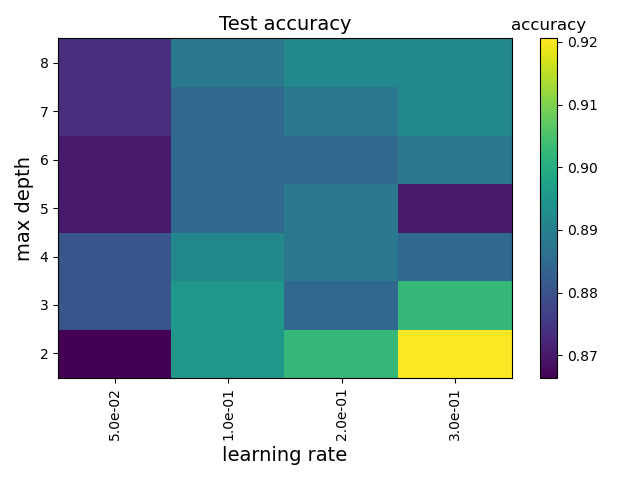
\includegraphics[scale=0.45]{../figures/xgboost/heatmaps/heatmap_nbins200_pca35_seed4155_ts0.20_accuracy_learning_rate_max_depth.png}
    \caption{Learning rate vs max depth}
  \end{subfigure}
  \begin{subfigure}{0.49\textwidth}
    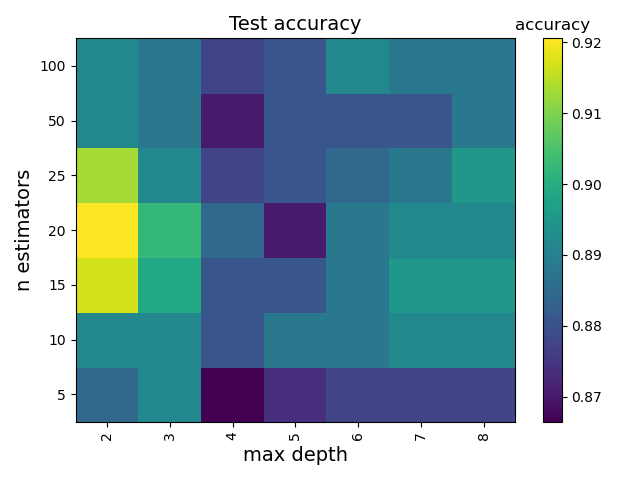
\includegraphics[scale=0.45]{../figures/xgboost/heatmaps/heatmap_nbins200_pca35_seed4155_ts0.20_accuracy_max_depth_n_estimators.png}
    \caption{Max depth vs n estimators}
  \end{subfigure}\\
  \begin{subfigure}{0.49\textwidth}
    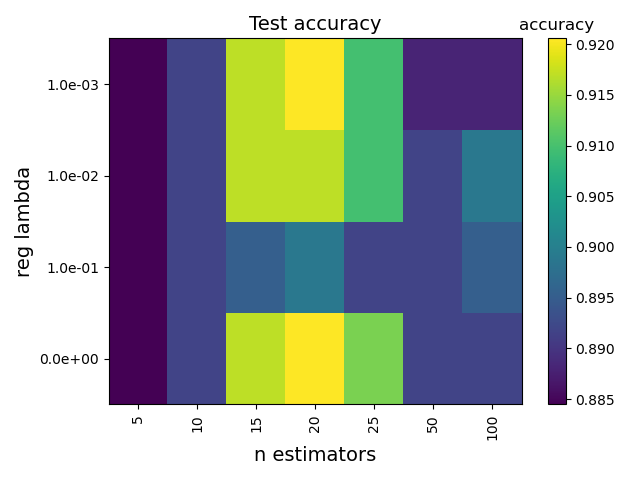
\includegraphics[scale=0.45]{../figures/xgboost/heatmaps/heatmap_nbins200_pca35_seed4155_ts0.20_accuracy_n_estimators_reg_lambda.png}
    \caption{Regularization vs n estimators}
  \end{subfigure}
  \begin{subfigure}{0.49\textwidth}
    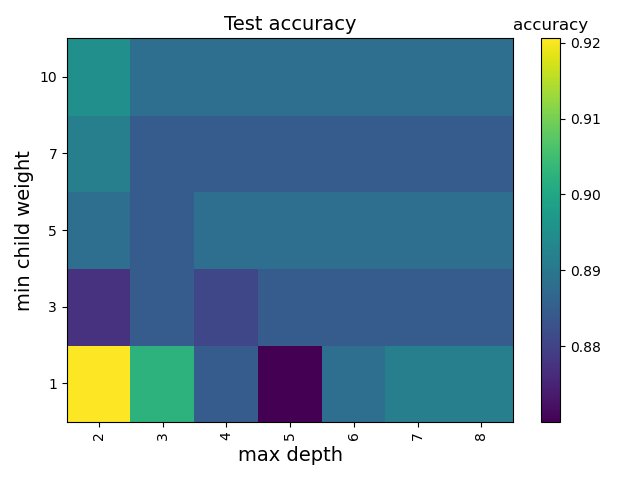
\includegraphics[scale=0.45]{../figures/xgboost/heatmaps/heatmap_nbins200_pca35_seed4155_ts0.20_accuracy_max_depth_min_child_weight.png}
    \caption{Max depth vs min child weight}
  \end{subfigure}
  \caption{Accuracy heatmaps for different hyperparameters. XGBoost, reduced data set. All other hyperparameters set to the best-fit from table \ref{tab:best_fit_xgboost_pca}.}
  \label{fig:app_xgboost_pca}
\end{figure}

\end{document}